% mainfile: ../../Refinement.tex
To gain more understanding of the \picalc{} we will use \findex{Stargazer}\cite{stargazer}. Stargazer is a visual simulator for \picalc{}. \refFig{pi_visualization_stargazer_code} shows the code listing of the process $P\define\procres{x}{(\procpar{\proccall{A_1}{x}}{\proccall{B_1}{x}})}$ where: $\procdef{A_1}{y}\define{}\out{y}{{}}.\proccall{A_2}{y}$ and $\procdef{B_1}{z}\define{}\inp{z}{{}}.\proccall{B_2}{z}$ in Stargazer syntax.
\begin{figure}[ht!]
\lstinputlisting[backgroundcolor=\color{white}]{listings/pi_visualization_stargazer.pi}
\caption{Stargazer code for the process $P$ .}
\label{pi_visualization_stargazer_code}
\end{figure}

Stargazer can visualize the reaction $\procres{x}{(\procpar{\proccall{A_1}{x}}{\proccall{B_1}{x}})} \transs{\tau} \procres{x}{(\procpar{\proccall{A_2}{x}}{\proccall{B_2}{x}})}$ as shown in
\refFig{pi_visualization_stargazer_Before_react} and \refFig{pi_visualization_stargazer_After_react}.
\begin{figure}[ht!]
	\centering
	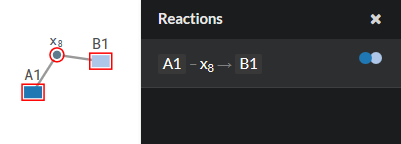
\includegraphics[width=0.5\textwidth]{./images/pi_visualization_stargazer_Before_react.png}
	\caption{The process $P$ before reaction occurrence.}
	\label{pi_visualization_stargazer_Before_react}
\end{figure}

\begin{figure}[ht!]
	\centering
	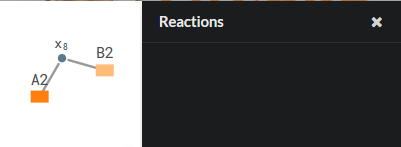
\includegraphics[width=0.5\textwidth]{./images/pi_visualization_stargazer_After_react.png}
	\caption{The process $P$ after reaction occurrence.}
	\label{pi_visualization_stargazer_After_react}
\end{figure}